%!TEX root = ../vernier.tex
\chapter{Related work} \label{sec:related}
Though SoftVis is a comparatively new field, AT\&T Bell Laboratory researchers were already working on visualizing changes in the evolution of software systems in 1992 \cite{seesoft}. Their objective in this particular project was to give project managers an overview of the state of complex systems and provide a tool that allows search for interesting trends and patterns in the development process. As shown in figure \ref{fig:seesoft}, they have used rectangles to represent files. The height of each rectangle represents the size of the file, and the pixels inside it represent lines of code. These pixel's colors represents the age of the last modification. Blue is used for lines that haven't been modified in a long time and red is used for recent changes.

\begin{figure}[H]
	\centering
	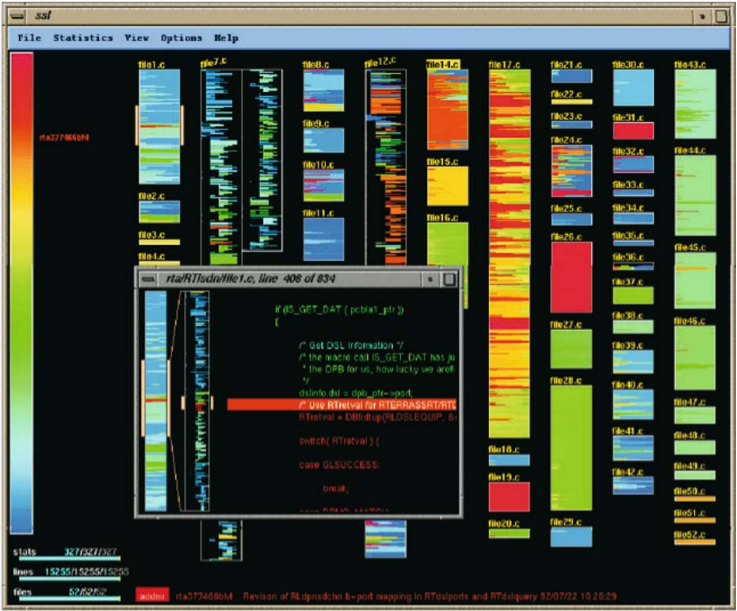
\includegraphics[width=1.0\textwidth]{figures/seesoft.png}
	\caption{}
	\label{fig:seesoft}
\end{figure}

SolidSX is tool designed for visually assisting Software Maintenance tasks. It integrates static code analysis and multiple linked views (e.g. treemaps, table lenses, and hierarchical edge bundles) in a single environment, allowing for insight about project structure, metrics and code dependencies.

\begin{figure}[H]
	\centering
	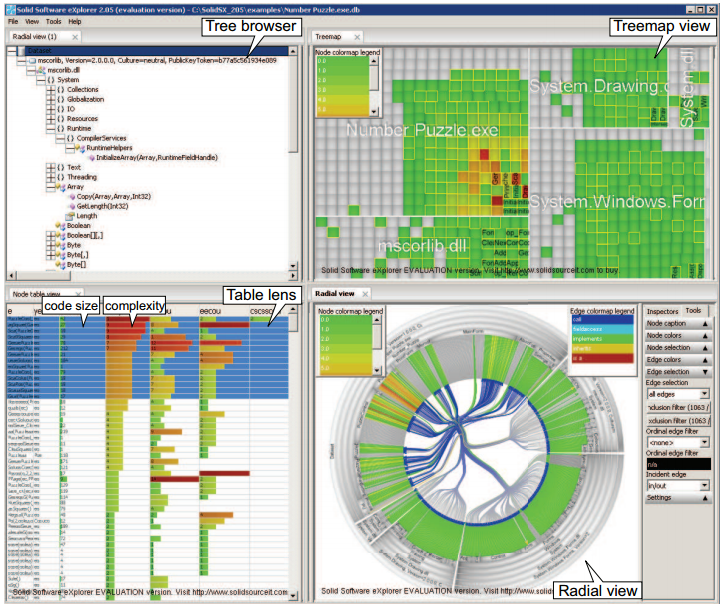
\includegraphics[width=1.0\textwidth]{figures/solidsx.png}
	\caption{}
	\label{fig:solidsx}
\end{figure}
